\begin{figure}
\centering
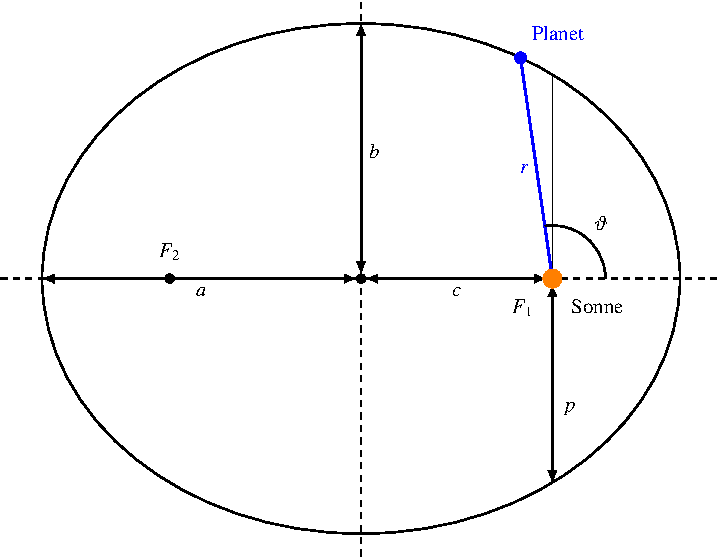
\includegraphics{papers/kepler/images/bahn.pdf}
\caption{Bahnellipse eines Planeten mit grosser Halbachse $a$ und
kleiner Halbachse $b$.
Die Sonne steht im Brennpunkt $F_1$.
Der zweite Brennpunkt $F_2$ bleibt leer.
Die Brennpunkte liegen im Abstand $c$ vom Mittelpunkt der Ellipse.
Der Halbparameter $p$ wird senkrecht zur grossen Achse gemessen.
Die durchgezogene Sehne durch $F_1$ liegt symmetrisch zur grossen Achse und steht deshalb senkrecht auf ihr.
Der Ort des Planeten wird durch den Abstand $r$ zur Sonne und den Polarwinkel $\vartheta$ beschrieben.
Der Winkel wird vom sonnennächsten Punkt aus gemessen.
\label{kepler:figure:ellipse}}
\end{figure}
